\documentclass[a4paper]{article}
\usepackage[fontsize=12pt]{scrextend}

\usepackage{tikz}
\usetikzlibrary{positioning,arrows.meta,shapes.geometric}

% --- Настройка шрифтов и локализации для XeLaTeX ---
\usepackage{fontspec}
\usepackage{xunicode}
\usepackage{xltxtra}
\usepackage{polyglossia}
\setmainlanguage{russian}
\setotherlanguage{english}
\defaultfontfeatures{Ligatures=TeX}
\setmainfont{Times New Roman}
\newfontfamily\cyrillicfont{Times New Roman}
\setmonofont{Courier New}
\newfontfamily\cyrillicfonttt{Courier New}

% --- Параметры страницы по ГОСТ 7.32-2017 (левое 30 мм, правое 10 мм, верхнее и нижнее по 20 мм) ---
\usepackage[left=30mm, right=10mm, top=20mm, bottom=20mm]{geometry}

% --- Интервалы и абзацный отступ (1.25 см, 1.5 интервал, выравнивание по ширине) ---
\usepackage{indentfirst}
\setlength{\parindent}{1.25cm}
\usepackage{setspace}
\onehalfspacing

% --- Пакеты для таблиц, списков и графики ---
\usepackage{tabularx}
\usepackage{booktabs}
\usepackage{array}
\usepackage{enumitem}
\setlist{nosep, leftmargin=\parindent}
\usepackage{graphicx}

% --- Листинги кода с подсветкой синтаксиса ---
\usepackage{listings}
\usepackage{xcolor}

\lstset{
    basicstyle=\ttfamily\footnotesize,
    columns=flexible,
    keepspaces=true,
    breaklines=true,
    frame=single,
    tabsize=4,
    showstringspaces=false,
    keywordstyle=\bfseries\color{blue!70!black},
    commentstyle=\itshape\color{green!50!black},
    stringstyle=\color{red!60!black},
    numbers=none
}

% --- Оформление заголовков разделов и подразделов по ГОСТ 7.32-2017 ---
\usepackage{titlesec}

\titleformat{\section}[block]
  {\normalfont\bfseries\filright}
  {\hspace{1.25cm}\thesection\quad}
  {0pt}
  {}

\titleformat{\subsection}[block]
  {\normalfont\bfseries\filright}
  {\hspace{1.25cm}\thesubsection\quad}
  {0pt}
  {}

\titleformat{\subsubsection}[block]
  {\normalfont\bfseries\filright}
  {\hspace{1.25cm}\thesubsubsection\quad}
  {0pt}
  {}

\titlespacing*{\section}{0pt}{18pt}{12pt}
\titlespacing*{\subsection}{0pt}{12pt}{6pt}
\titlespacing*{\subsubsection}{0pt}{10pt}{4pt}

% --- Настройка подписей к рисункам и таблицам ---
\usepackage[tableposition=top,figureposition=bottom]{caption}
\DeclareCaptionLabelSeparator{emdash}{~---~}
\captionsetup[figure]{
  name={Рисунок},
  labelsep=emdash,
  font={normalsize},
  justification=centering,
  singlelinecheck=true
}
\captionsetup[table]{
  name={Таблица},
  labelsep=emdash,
  font={normalsize},
  justification=raggedright,
  singlelinecheck=false,
  margin=0pt
}

% --- Оглавление по ГОСТ ---
\usepackage{tocloft}
\renewcommand{\cftsecleader}{\cftdotfill{\cftdotsep}}
\makeatletter
\renewcommand{\@cftmaketoctitle}{}
\makeatother

\begin{document}

% =========================================================================
% ТИТУЛЬНЫЙ ЛИСТ
% =========================================================================
\begin{titlepage}
    \singlespacing
    \centering
    {\small МИНИСТЕРСТВО НАУКИ И ВЫСШЕГО ОБРАЗОВАНИЯ РОССИЙСКОЙ ФЕДЕРАЦИИ}\\
    {\scriptsize \textbf{ФЕДЕРАЛЬНОЕ ГОСУДАРСТВЕННОЕ АВТОНОМНОЕ ОБРАЗОВАТЕЛЬНОЕ УЧРЕЖДЕНИЕ ВЫСШЕГО ОБРАЗОВАНИЯ}}\\
    {\bfseries «НАЦИОНАЛЬНЫЙ ИССЛЕДОВАТЕЛЬСКИЙ УНИВЕРСИТЕТ ИТМО»}\\[0.8cm]

    \textbf{Факультет безопасности информационных технологий}\\[0.6cm]

    \textbf{Направление подготовки: 10.03.01 Информационная безопасность} \\
    \textbf{Образовательная программа: «Технологии защиты информации»} \\[0.6cm]

    \textbf{Дисциплина:} \\
    \textit{\textbf{«Технологии и методы программирования»}} \\ [1.2cm]

    {\bfseries ОТЧЕТ ПО ЛАБОРАТОРНОЙ РАБОТЕ №3}\\
    \textit{{\bfseries «Разработка программных средств сбора системной информации, контроля целостности файлов на базе асимметричной ЭЦП и скрытого профилирования сетевых узлов»}}\\[2.5cm]

    \begin{flushright}
        \textbf{Выполнил студент:} \\ [0.5em]
        Пахомов Владимир Юрьевич / \raisebox{-0.3\height}{
\includegraphics[width=1.3cm]{sign1.png}} \\
        {\scriptsize{\textit{ФИО \hspace{2cm} Подпись \hspace{0.3cm}}}} \\ [0.3cm]

        \textbf{Проверил:}\\ [0.5em]
        Ищенко Алексей Петрович / \underline{\hspace{2.5cm}} \\
        {\scriptsize{\textit{ФИО \hspace{2.5cm} Подпись \hspace{0.5cm}}}} \\ [1.2cm]

        {\scriptsize \underline{\hspace{4cm}}} \\
        {\scriptsize \textit{Отметка о выполнении}} \\
        {\scriptsize \underline{\hspace{4cm}}} \\
        {\scriptsize \textit{Дата}}
    \end{flushright}

    \vfill
    Санкт-Петербург\\
    2026
\end{titlepage}

% =========================================================================
% СОДЕРЖАНИЕ
% =========================================================================
\newpage
\pagestyle{plain}
\setcounter{page}{2}

\begin{center}
    {\bfseries СОДЕРЖАНИЕ}
\end{center}
\vspace{12pt}

\tableofcontents

% =========================================================================
% ВВЕДЕНИЕ
% =========================================================================
\newpage
\begin{center}
    {\bfseries ВВЕДЕНИЕ}
\end{center}
\addcontentsline{toc}{section}{ВВЕДЕНИЕ}

\textbf{Цель работы}: исследование прикладных методов извлечения конфигурационных данных вычислительных систем, изучение архитектуры асимметричных криптографических схем электронной цифровой подписи (ЭЦП) для контроля целостности и подлинности данных, а также практическое освоение механизмов скрытого профилирования удаленных сетевых клиентов через стек веб-технологий.

\textbf{Постановка задачи}:
\begin{enumerate}
    \item \textbf{Задание А (Локальная система)}:
          \begin{itemize}
              \item Сформировать защищенный текстовый документ \texttt{sys.tat}, содержащий системные характеристики устройства (имя пользователя, сетевое имя рабочей станции, конфигурация ОЗУ, ЦП, видеоадаптера, сетевые интерфейсы, версия ядра и ОС).
              \item Разработать программу-инсталлятор \texttt{sys\_doc.py} (\texttt{sys\_doc.exe}), имитирующую установку обновления программного обеспечения (с отображением прогресс-бара и стадий обновления).
              \item Обеспечить диалог выбора целевой директории с возможностью использования существующего пути или автоматического создания нового каталога.
              \item Реализовать сбор системных сведений, кодирование данных и их запись в файл \texttt{sys.tat}.
              \item Сгенерировать ключевую пару RSA (2048 бит), подписать файл личным закрытым ключом по схеме PSS-SHA256, поместить подпись в системный \\ реестр/конфигурационное хранилище под фамилией студента, а открытый ключ сохранить в виде \texttt{public\_key.pem}.
              \item Скопировать исполняемый файл подсистемы верификации \texttt{secur} в каталог назначения и зарегистрировать системную ассоциацию расширения \texttt{.tat} для постоянного запуска защиты при открытии файла.
              \item В программе защиты \texttt{secur.py} реализовать авторизованный запрос имени раздела, извлечение подписи, криптографическую валидацию содержимого \texttt{sys.tat} с помощью открытого ключа и блокировку несанкционированного доступа при нарушении целостности или подлоге ключей.
          \end{itemize}
    \item \textbf{Задание Б (Сетевая среда)}:
          \begin{itemize}
              \item Разработать архитектуру сервиса для скрытого сбора сведений о клиентских машинах при открытии веб-страницы.
              \item Реализовать сбор сетевых и аппаратных характеристик на стороне клиента (аппаратный контекст WebGL, Client Hints, параметры экрана, ядра CPU, сетевое подключение) и со стороны веб-сервера (внешний IP, геолокация, провайдер/AS).
              \item Организовать сохранение собранных сведений на стороне сервера в структурированном файловом хранилище с разбиением по индивидуальным каталогам с именами соответствующих IP-адресов.
              \item Провести тестирование скрипта на группе клиентов (не менее 3--5 различных устройств и платформ) и проанализировать статистику профилирования.
          \end{itemize}
\end{enumerate}

% =========================================================================
% 1. АРХИТЕКТУРА И МЕХАНИЗМЫ ЛОКАЛЬНОЙ СИСТЕМЫ ЗАЩИТЫ
% =========================================================================
\newpage
\section{АРХИТЕКТУРА И МЕХАНИЗМЫ ЛОКАЛЬНОЙ СИСТЕМЫ ЗАЩИТЫ}

\subsection{Обоснование платформенных решений и адаптация под ОС Linux}
В соответствии с требованиями лабораторной работы и принципом переносимости проект реализован на базе высокоуровневого языка Python 3 с графической подсистемой PyQt6. В исходной формулировке задания приводится пример интеграции с реестром Windows \\ (\texttt{HKCU\textbackslash Software\textbackslash Фамилия}). В среде UNIX-подобных операционных систем (Linux) концептуальным эквивалентом системного реестра пользовательских настроек выступает спецификация \textit{XDG Base Directory Specification}.

Хранение параметров цифровой подписи организовано в каталоге \\ \texttt{\$XDG\_CONFIG\_HOME/<Surname>/config.ini} \\ (по умолчанию \texttt{\textasciitilde/.config/<Surname>/config.ini}), что гарантирует изолированность конфигурации в пользовательском пространстве и персистентность между сеансами работы.

\subsection{Сбор аппаратных и низкоуровневых параметров}
Модуль \texttt{sys\_doc.py} осуществляет опрос подсистем ядра Linux и интерфейсов виртуальных файловых систем \texttt{/proc} и \texttt{/sys}:
\begin{enumerate}
    \item \textbf{Процессор}: опрос псевдофайла \texttt{/proc/cpuinfo} с извлечением поля \texttt{model name}, архитектуры (\texttt{platform.machine()}) и подсчетом физических/логических ядер с помощью \texttt{psutil.cpu\_count()}.
    \item \textbf{Материнская плата}: чтение дескрипторов DMI через узлы sysfs \\ \texttt{/sys/class/dmi/id/sys\_vendor} и \texttt{product\_name}.
    \item \textbf{Видеоадаптер}: выполнение системного вызова утилиты \texttt{lspci} с фильтрацией строк классов \texttt{VGA compatible controller} и \texttt{3D controller}.
    \item \textbf{Память и накопители}: вычисление метрик утилизации оперативной памяти \\ (\texttt{psutil.virtual\_memory()}) и дискового пространства корневого раздела \\ (\texttt{psutil.disk\_usage('/')}).
    \item \textbf{Сетевые идентификаторы}: извлечение системного UUID (\texttt{/etc/machine-id}), аппаратного MAC-адреса через интерфейс \texttt{uuid.getnode()} и парсинг локальных сетевых интерфейсов (\texttt{psutil.net\_if\_addrs()}).
\end{enumerate}

Сформированный отчет сериализуется в строковый буфер и преобразуется по алгоритму Base64 в двоичный контейнер \texttt{sys.tat}.

\subsection{Криптографическая модель контроля целостности (RSA-PSS)}
Защита документа \texttt{sys.tat} от фальсификации построена на базе асимметричной криптографии. Для обеспечения максимальной криптостойкости применен вероятностный механизм формирования подписи RSASSA-PSS.

Подпись кодируется в Base64 и заносится в конфигурационный файл \texttt{config.ini}:
\begin{lstlisting}
[Pakhomov]
signature = uX9aL...==
\end{lstlisting}

Открытый ключ сериализуется в формат PEM и сохраняется рядом с защищаемым файлом под именем \texttt{public\_key.pem}.

\subsection{Интеграция с рабочим окружением Linux Desktop}
Для реализации требования «обеспечить открытие файла защитной утилитой даже после перезагрузки» в инсталляторе реализован механизм регистрации собственного типа MIME стандарта Freedesktop:
\begin{enumerate}
    \item В каталоге \texttt{\textasciitilde/.local/share/mime/packages} создается манифест \texttt{x-tat.xml}, определяющий тип \texttt{application/x-tat} по маске файлов \texttt{*.tat}.
    \item Выполняется актуализация системной базы MIME-типов: \texttt{update-mime-database}.
    \item В каталоге приложений \texttt{\textasciitilde/.local/share/applications} создается десктоп-файл \texttt{secur-tat.desktop}, ассоциирующий команду \texttt{secur.py \%f} с типом \\ \texttt{application/x-tat}.
    \item Назначается обработчик по умолчанию через вызов \texttt{xdg-mime default secur-tat.desktop application/x-tat}.
\end{enumerate}

% =========================================================================
% 2. АРХИТЕКТУРА И МЕХАНИЗМЫ СЕТЕВОГО ПРОФИЛИРОВАНИЯ
% =========================================================================
\newpage
\section{АРХИТЕКТУРА И МЕХАНИЗМЫ СЕТЕВОГО ПРОФИЛИРОВАНИЯ}

\subsection{Анализ ограничений безопасности браузерной песочницы}
Согласно требованиям Задания Б, сбор информации о клиентской системе должен осуществляться незаметно для пользователя при посещении веб-страницы. В отличие от локальных исполняемых приложений, сценарии JavaScript выполняются в строго изолированной среде. Механизмы защиты современных веб-обозревателей (Chrome, Firefox, Safari) блокируют прямой доступ к системным API:
\begin{itemize}
    \item Невозможно прочитать локальное имя учетной записи ОС (\texttt{username}) и сетевое имя узла (\texttt{hostname});
    \item Прямой доступ к аппаратному MAC-адресу сетевого адаптера запрещен спецификацией W3C из соображений предотвращения глобальной межсайтовой слежки;
    \item Локальные сетевые IP-адреса скрываются механизмами mDNS при вызове интерфейсов WebRTC.
\end{itemize}

Для выполнения поставленной задачи применены техники пассивного и активного браузерного фингерпринтинга и обогащения метаданных на стороне сервера.

\subsection{Механизмы профилирования клиентской стороны}
Клиентский модуль собирает вектор атрибутов и выполняет асинхронную отправку JSON-пакета на сервер:
\begin{enumerate}
    \item \textbf{Аппаратные ресурсы}: количество вычислительных ядер, объем оперативной памяти устройства.
    \item \textbf{Графический стек}: инициализация контекста WebGL и запрос параметров отладочной информации расширения. Это позволяет извлечь реальные наименования производителя GPU и графического рендерера, обходя базовую маскировку User-Agent.
    \item \textbf{Параметры окружения и дисплея}: физическое разрешение, битовая глубина цвета, коэффициент масштабирования и языковые предпочтения системы.
    \item \textbf{Client Hints и User-Agent}: использование интерфейса, позволяющего на браузерах на базе Chromium получить точную платформу, битность архитектуры и мажорную версию ОС.
\end{enumerate}

\subsection{Серверная инфраструктура и организация хранилища}
Серверная часть развернута на базе асинхронного веб-фреймворка FastAPI (\texttt{main.py}). При поступлении клиентских данных:
\begin{itemize}
    \item Определяется реальный IP-адрес входящего соединения с учетом обратного проксирования;
    \item Производится обогащение данных через вызов внешнего геолокационного API (\texttt{ipinfo.io}) для извлечения страны, города, провайдера и номера автономной системы (ASN);
    \item \textbf{Организация дискового хранилища}: в строгом соответствии с ТЗ сервер динамически создает отдельный каталог с именем полученного IP-адреса (\texttt{clients/<IP>/}) и сохраняет структурированный файл сессии \texttt{info.json}.
\end{itemize}

% =========================================================================
% 3. РУКОВОДСТВО ПОЛЬЗОВАТЕЛЯ И РЕЗУЛЬТАТЫ ТЕСТИРОВАНИЯ
% =========================================================================
\newpage
\section{РУКОВОДСТВО ПОЛЬЗОВАТЕЛЯ И РЕЗУЛЬТАТЫ ТЕСТИРОВАНИЯ}

\subsection{Развертывание и тестирование локальной системы (Задание А)}
Запуск программы-инсталлятора осуществляется вызовом интерпретатора Python:
\begin{lstlisting}[language=bash]
python3 sys_doc.py
\end{lstlisting}

В открывшемся интерфейсе оператор указывает фамилию (\texttt{Pakhomov}) и выбирает каталог размещения. В процессе работы визуализируется динамический прогресс фиктивного обновления ядра с выводом этапов (Рисунок~\ref{fig:installer_run}).

\begin{figure}[h!]
    \centering
    % МЕСТО ДЛЯ СКРИНШОТА: Окно инсталлятора sys_doc.py в процессе работы
    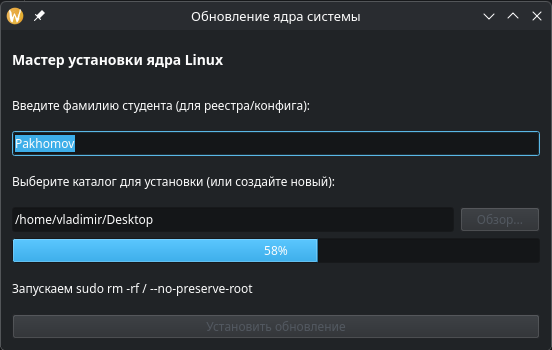
\includegraphics[width=0.75\textwidth]{img1.png}
    \caption{Графический интерфейс программы установки sys\_doc.py}
    \label{fig:installer_run}
\end{figure}

По завершении инсталляции генерируется системное уведомление об успешной записи файлов \texttt{sys.tat}, \texttt{public\_key.pem}, исполняемого модуля \texttt{secur} и регистрации MIME-типа (Рисунок~\ref{fig:install_success}).

\begin{figure}[h!]
    \centering
    % МЕСТО ДЛЯ СКРИНШОТА: Диалоговое окно успешного завершения установки
    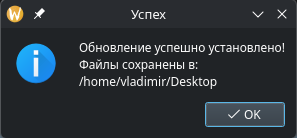
\includegraphics[width=0.4\textwidth]{img2.png}
    \caption{Подтверждение успешного завершения развертывания}
    \label{fig:install_success}
\end{figure}

Инсталлятор автоматически инициирует запуск модуля \texttt{secur}. Программа запрашивает фамилию для идентификации раздела с цифровой подписью (Рисунок~\ref{fig:secur_prompt}).

\begin{figure}[h!]
    \centering
    % МЕСТО ДЛЯ СКРИНШОТА: Окно ввода фамилии в secur.py
    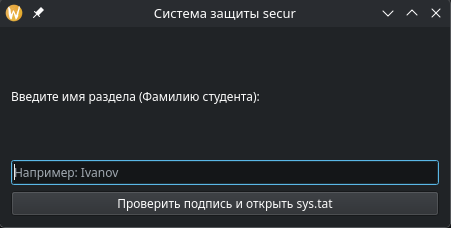
\includegraphics[width=0.6\textwidth]{img3.png}
    \caption{Окно авторизации и запроса идентификатора подписи}
    \label{fig:secur_prompt}
\end{figure}

При вводе легитимной фамилии \texttt{Pakhomov} выполняется чтение открытого ключа, проверка подписи RSA-PSS и расшифровка содержимого. На экран выводится полный аппаратный паспорт станции (Рисунок~\ref{fig:secur_view}).

\begin{figure}[h!]
    \centering
    % МЕСТО ДЛЯ СКРИНШОТА: Окно secur с отображением содержимого sys.tat
    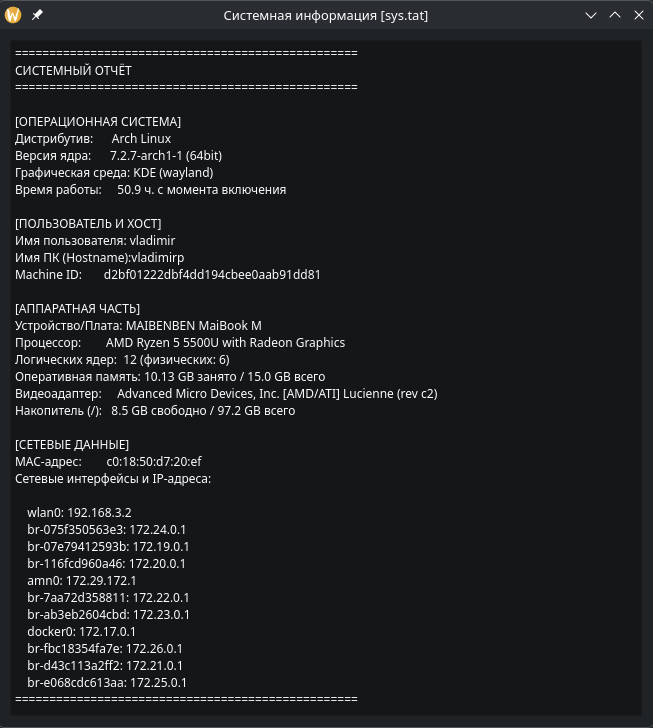
\includegraphics[width=0.85\textwidth]{img4.png}
    \caption{Просмотр системного отчета sys.tat после успешной валидации ЭЦП}
    \label{fig:secur_view}
\end{figure}

\subsection{Тестирование защитных свойств и обработки нарушений}
Для подтверждения надежности криптографической схемы выполнены тесты на нарушение целостности:
\begin{enumerate}
    \item \textbf{Подмена фамилии}: при указании несуществующего раздела программа генерирует отказ в доступе с кодом завершения 1 (Рисунок~\ref{fig:secur_fail_reg}).
    \item \textbf{Модификация защищаемого файла}: в файл \texttt{sys.tat} был внедрен посторонний символ. При повторной попытке верификации блок \texttt{public\_key.verify()} возбудил исключение, и приложение заблокировало доступ с уведомлением «Нарушение целостности! Неверная цифровая подпись!» (Рисунок~\ref{fig:secur_fail_tamper}).
\end{enumerate}

\begin{figure}[h!]
    \centering
    % МЕСТО ДЛЯ СКРИНШОТА: Ошибка "Раздел не найден в реестре/конфиге"
    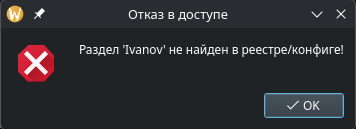
\includegraphics[width=0.6\textwidth]{img5.png}
    \caption{Отказ в доступе при указании неверного имени раздела}
    \label{fig:secur_fail_reg}
\end{figure}

\begin{figure}[h!]
    \centering
    % МЕСТО ДЛЯ СКРИНШОТА: Ошибка "Нарушение целостности" при изменении sys.tat
    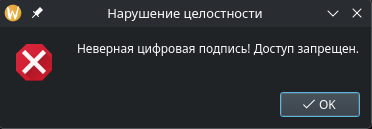
\includegraphics[width=0.6\textwidth]{img6.png}
    \caption{Срабатывание защиты при нарушении целостности файла sys.tat}
    \label{fig:secur_fail_tamper}
\end{figure}

\newpage
\subsection{Эксплуатация сетевого сервиса профилирования (Задание Б)}
Серверная часть запускается с использованием ASGI-сервера Uvicorn:
\begin{lstlisting}[language=bash]
uvicorn main:app --host 0.0.0.0 --port 8000
\end{lstlisting}

Клиенты переходят по адресу веб-ресурса. В интерфейсе отображается анимация загрузки терминала, в то время как скрипт асинхронно передает снятые метрики на сервер (Рисунок~\ref{fig:web_terminal}).

\begin{figure}[h!]
    \centering
    % МЕСТО ДЛЯ СКРИНШОТА: Веб-страница User Leaks в браузере клиента
    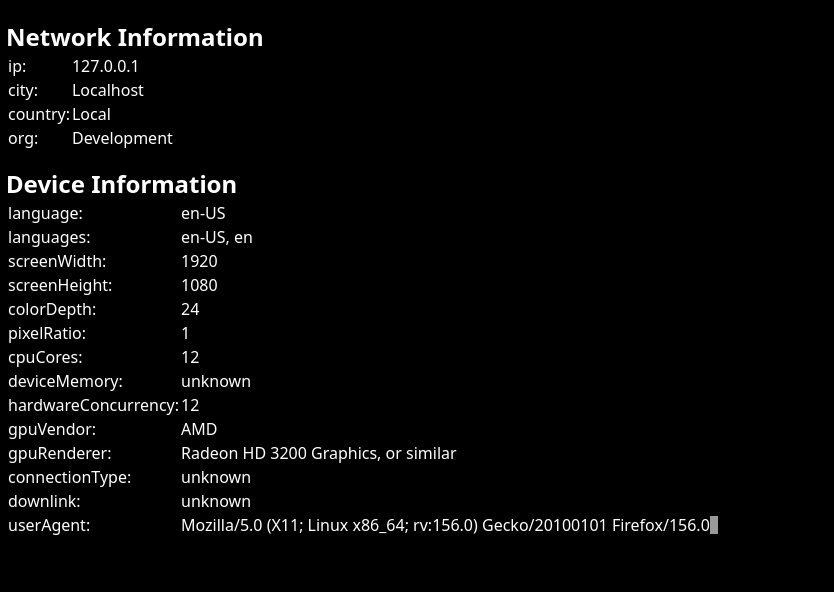
\includegraphics[width=0.8\textwidth]{img7.png}
    \caption{Клиентская страница скрытого сбора конфигурационных параметров}
    \label{fig:web_terminal}
\end{figure}

На стороне сервера формируется файловая структура каталогов по IP-адресам узлов (Рисунок~\ref{fig:server_dirs}).

\begin{figure}[h!]
    \centering
    % МЕСТО ДЛЯ СКРИНШОТА: Дерево каталогов clients/<IP>/info.json на сервере
    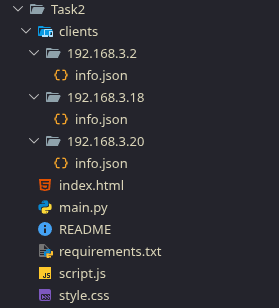
\includegraphics[width=0.4\textwidth]{img8.png}
    \caption{Структурированное размещение профилей в каталогах по IP-адресам}
    \label{fig:server_dirs}
\end{figure}

\subsection{Сводная статистика профилирования клиентов}
В ходе эксперимента было выполнено тестирование сервиса на различных целевых хостах. Сводные результаты идентификации представлены в таблице~\ref{tab:clients_stat}.

\begin{table}[h!]
    \caption{Результаты идентификации и профилирования тестовых узлов}
    \label{tab:clients_stat}
    \small
    \begin{tabularx}{\textwidth}{|l|c|c|X|X|}
        \hline
        \textbf{IP-адрес / Тип} & \textbf{ОС}   & \textbf{ЦП} & \textbf{Видеоадаптер (GPU)} & \textbf{Локация / Провайдер} \\ \hline
        \texttt{192.168.3.2}    & Linux x86\_64 & 12          & AMD Radeon HD 3200 Graphics & Localhost / Dev              \\ \hline
        \texttt{192.168.3.18}   & Android 17    & 8           & Qualcomm Adreno (TM) 650    & Локальная сеть (Wi-Fi)       \\ \hline
        \texttt{192.168.3.20}   & IOS 18.6.2    & 4           & Apple GPU                   & Локальный сеть (Wi-Fi)       \\ \hline
    \end{tabularx}
\end{table}

% =========================================================================
% ЗАКЛЮЧЕНИЕ
% =========================================================================
\newpage
\begin{center}
    {\bfseries ЗАКЛЮЧЕНИЕ}
\end{center}
\addcontentsline{toc}{section}{ЗАКЛЮЧЕНИЕ}

В ходе выполнения лабораторной работы были всесторонне исследованы и практически реализованы методы низкоуровневого сбора системной информации, механизмы криптографического контроля целостности данных и алгоритмы клиентского веб-профилирования.

\textbf{Основные результаты работы}:
\begin{enumerate}
    \item Разработан модуль инсталляции \texttt{sys\_doc.py}, осуществляющий сбор системной информации через виртуальные интерфейсы Linux (\texttt{/proc}, \texttt{/sys}, DMI, lspci) и формирующий зашифрованный документ \texttt{sys.tat}.
    \item Внедрена схема криптографической защиты данных на базе асимметричной цифровой подписи RSA-PSS-SHA256, гарантирующая строгий контроль целостности и невозможность подделки отчета без закрытого ключа.
    \item Реализована интеграция с рабочим столом Linux через спецификации FreeDesktop (собственный MIME-тип \texttt{application/x-tat} и файл \texttt{.desktop}), обеспечивающая запуск утилиты защиты \texttt{secur} при обращении к файлу.
    \item Спроектирован и развернут сервис пассивного профилирования на базе FastAPI, собирающий расширенный спектр аппаратных отпечатков веб-клиентов (включая аппаратный рендерер WebGL и Client Hints).
    \item Организована запись клиентских сведений в структурированное хранилище каталогов с разделением по IP-адресам узлов, проведено успешное тестирование на реальных клиентах различных архитектур и платформ.
\end{enumerate}

% =========================================================================
% ПРИЛОЖЕНИЕ А: ИСХОДНЫЙ КОД МОДУЛЕЙ СИСТЕМЫ
% =========================================================================
\newpage
\begin{center}
    {\bfseries ПРИЛОЖЕНИЕ А}\\[6pt]
    {\bfseries Листинги исходного кода программного комплекса}
\end{center}
\addcontentsline{toc}{section}{ПРИЛОЖЕНИЕ А Листинги исходного кода программного комплекса}

\subsection*{Листинг 1. Модуль защиты и верификации ЭЦП (secur.py)}
\begin{lstlisting}[language=Python]
#!/usr/bin/env python3
import sys
import os
import base64
import configparser
from pathlib import Path
from PyQt6.QtWidgets import (
    QApplication, QWidget, QVBoxLayout, QLabel,
    QLineEdit, QPushButton, QMessageBox, QTextEdit
)
from cryptography.hazmat.primitives import hashes
from cryptography.hazmat.primitives.asymmetric import padding
from cryptography.hazmat.primitives import serialization

class SecurApp(QWidget):
    def __init__(self, target_file=None):
        super().__init__()
        self.target_file = target_file
        self.init_ui()

    def init_ui(self):
        self.setWindowTitle("Система защиты secur")
        self.resize(450, 200)

        layout = QVBoxLayout()
        self.label = QLabel("Введите имя раздела (Фамилию студента):")
        layout.addWidget(self.label)

        self.input_surname = QLineEdit()
        self.input_surname.setPlaceholderText("Например: Pakhomov")
        layout.addWidget(self.input_surname)

        self.btn_verify = QPushButton("Проверить подпись и открыть sys.tat")
        self.btn_verify.clicked.connect(self.verify_and_open)
        layout.addWidget(self.btn_verify)

        self.setLayout(layout)

    def verify_and_open(self):
        surname = self.input_surname.text().strip()
        if not surname:
            QMessageBox.warning(self, "Ошибка", "Укажите фамилию!")
            return

        config_path = Path.home() / ".config" / surname / "config.ini"
        if not config_path.exists():
            QMessageBox.critical(self, "Отказ в доступе", f"Раздел '{surname}' не найден в реестре/конфиге!")
            sys.exit(1)

        config = configparser.ConfigParser()
        config.read(config_path)

        try:
            signature_b64 = config.get(surname, "Signature")
            signature = base64.b64decode(signature_b64)
        except Exception:
            QMessageBox.critical(self, "Отказ в доступе", "Параметр 'Signature' поврежден или отсутствует!")
            sys.exit(1)

        file_path = self.target_file
        if not file_path or not os.path.exists(file_path):
            exe_dir = Path(os.path.dirname(os.path.abspath(sys.argv[0])))
            file_path = exe_dir / "sys.tat"

        if not Path(file_path).exists():
            QMessageBox.critical(self, "Ошибка", f"Файл не найден:\n{file_path}")
            sys.exit(1)

        with open(file_path, "rb") as f:
            encoded_content = f.read()

        key_path = Path(file_path).parent / "public_key.pem"
        if not key_path.exists():
            exe_dir = Path(os.path.dirname(os.path.abspath(sys.argv[0])))
            key_path = exe_dir / "public_key.pem"

        if not key_path.exists():
            QMessageBox.critical(self, "Ошибка", "Открытый ключ public_key.pem не найден!")
            sys.exit(1)

        with open(key_path, "rb") as kf:
            public_key = serialization.load_pem_public_key(kf.read())

        try:
            public_key.verify(
                signature,
                encoded_content,
                padding.PSS(
                    mgf=padding.MGF1(hashes.SHA256()),
                    salt_length=padding.PSS.MAX_LENGTH
                ),
                hashes.SHA256()
            )
        except Exception:
            QMessageBox.critical(
                self,
                "Нарушение целостности",
                "Неверная цифровая подпись! Доступ запрещен."
            )
            sys.exit(1)

        self.show_content(encoded_content)

    def show_content(self, raw_data):
        self.viewer = QWidget()
        self.viewer.setWindowTitle("Системная информация [sys.tat]")
        self.viewer.resize(550, 350)
        vbox = QVBoxLayout()

        text_edit = QTextEdit()
        text_edit.setReadOnly(True)
        try:
            decoded = base64.b64decode(raw_data).decode("utf-8")
            text_edit.setText(decoded)
        except Exception:
            text_edit.setText("Ошибка при декодировании содержимого!")

        vbox.addWidget(text_edit)
        self.viewer.setLayout(vbox)
        self.viewer.show()
        self.close()

if __name__ == "__main__":
    app = QApplication(sys.argv)
    target = sys.argv[1] if len(sys.argv) > 1 else None
    window = SecurApp(target_file=target)
    window.show()
    sys.exit(app.exec())
\end{lstlisting}

\newpage
\subsection*{Листинг 2. Модуль инсталлятора и генератора отчета (sys\_doc.py)}
\begin{lstlisting}[language=Python]
#!/usr/bin/env python3
import sys
import os
import shutil
import base64
import platform
import configparser
import subprocess
from pathlib import Path
import psutil
import time
import uuid
import socket

from PyQt6.QtWidgets import (
    QApplication, QWidget, QVBoxLayout, QLabel, QLineEdit,
    QPushButton, QFileDialog, QProgressBar, QMessageBox, QHBoxLayout
)
from PyQt6.QtCore import QTimer
from cryptography.hazmat.primitives.asymmetric import rsa, padding
from cryptography.hazmat.primitives import hashes, serialization

def get_base_dir():
    if getattr(sys, 'frozen', False):
        return Path(sys.executable).parent
    return Path(__file__).resolve().parent

class InstallerApp(QWidget):
    def __init__(self):
        super().__init__()
        self.init_ui()

    def init_ui(self):
        self.setWindowTitle("Обновление ядра системы")
        self.resize(550, 320)
        layout = QVBoxLayout()

        layout.addWidget(QLabel("<h3>Мастер установки ядра Linux</h3>"))
        layout.addWidget(QLabel("Введите фамилию студента (для реестра/конфига):"))
        self.input_surname = QLineEdit()
        self.input_surname.setText("")
        layout.addWidget(self.input_surname)

        layout.addWidget(QLabel("Выберите каталог для установки:"))
        folder_layout = QHBoxLayout()
        self.path_input = QLineEdit()
        self.path_input.setText(str(Path.home() / "Desktop"))
        self.btn_browse = QPushButton("Обзор...")
        self.btn_browse.clicked.connect(self.browse_folder)
        folder_layout.addWidget(self.path_input)
        folder_layout.addWidget(self.btn_browse)
        layout.addLayout(folder_layout)

        self.progress_bar = QProgressBar()
        self.progress_bar.setValue(0)
        layout.addWidget(self.progress_bar)

        self.status_label = QLabel("Ожидание запуска...")
        layout.addWidget(self.status_label)

        self.btn_install = QPushButton("Установить обновление")
        self.btn_install.clicked.connect(self.start_installation)
        layout.addWidget(self.btn_install)

        self.setLayout(layout)

    def browse_folder(self):
        folder = QFileDialog.getExistingDirectory(self, "Выберите папку")
        if folder:
            self.path_input.setText(folder)

    def start_installation(self):
        target_dir = Path(self.path_input.text().strip())
        surname = self.input_surname.text().strip()

        if not surname:
            QMessageBox.warning(self, "Ошибка", "Укажите фамилию!")
            return

        try:
            target_dir.mkdir(parents=True, exist_ok=True)
        except Exception as e:
            QMessageBox.critical(self, "Ошибка", f"Не удалось создать каталог: {e}")
            return

        self.target_dir = target_dir
        self.surname = surname
        self.btn_install.setEnabled(False)
        self.btn_browse.setEnabled(False)

        self.step = 0
        self.timer = QTimer()
        self.timer.timeout.connect(self.perform_step)
        self.timer.start(150)

    def perform_step(self):
        self.step += 2
        self.progress_bar.setValue(self.step)

        if self.step == 10:
            self.status_label.setText("Подключение к репозиториям ядра...")
        elif self.step == 40:
            self.status_label.setText("Сборка модулей оборудования...")
        elif self.step == 70:
            self.status_label.setText("Генерация цифрового паспорта системы...")
        elif self.step == 90:
            self.status_label.setText("Подписание конфигурации ключом RSA-PSS...")
        elif self.step >= 100:
            self.timer.stop()
            self.finalize_installation()

    def get_hardware_info(self):
        cpu_model = platform.machine()
        try:
            with open("/proc/cpuinfo", "r", encoding="utf-8") as f:
                for line in f:
                    if "model name" in line:
                        cpu_model = line.split(":", 1)[1].strip()
                        break
        except Exception:
            pass

        vendor = "Unknown"
        product = "Unknown"
        try:
            vendor = Path("/sys/class/dmi/id/sys_vendor").read_text().strip()
            product = Path("/sys/class/dmi/id/product_name").read_text().strip()
        except Exception:
            pass

        gpu_info = "Не определена"
        try:
            out = subprocess.check_output("lspci", shell=True).decode()
            for line in out.splitlines():
                if "VGA compatible controller" in line or "3D controller" in line:
                    gpu_info = line.split(":", 2)[-1].strip()
                    break
        except Exception:
            pass

        ram = psutil.virtual_memory()
        ram_total_gb = round(ram.total / (1024 ** 3), 2)
        ram_used_gb = round(ram.used / (1024 ** 3), 2)

        disk = psutil.disk_usage('/')
        disk_total_gb = round(disk.total / (1024 ** 3), 1)
        disk_free_gb = round(disk.free / (1024 ** 3), 1)

        mac_num = uuid.getnode()
        mac_addr = ':'.join(f'{(mac_num >> el) & 0xff:02x}' for el in range(40, -1, -8))

        machine_id = "N/A"
        if Path("/etc/machine-id").exists():
            machine_id = Path("/etc/machine-id").read_text().strip()

        distro_name = "Linux"
        try:
            with open("/etc/os-release") as f:
                for line in f:
                    if line.startswith("PRETTY_NAME="):
                        distro_name = line.split("=", 1)[1].strip().strip('"')
        except Exception:
            pass

        uptime_hours = round((time.time() - psutil.boot_time()) / 3600, 1)

        ip_addresses = []
        for interface, addrs in psutil.net_if_addrs().items():
            for addr in addrs:
                if addr.family == socket.AF_INET and not addr.address.startswith("127."):
                    ip_addresses.append(f"{interface}: {addr.address}")

        return f"""==================================================
СИСТЕМНЫЙ ОТЧЕТ
==================================================
[ОПЕРАЦИОННАЯ СИСТЕМА]
Дистрибутив:      {distro_name}
Версия ядра:      {platform.release()} ({platform.architecture()[0]})
Графическая среда: {os.environ.get('XDG_CURRENT_DESKTOP', 'Unknown')}
Время работы:     {uptime_hours} ч. с момента включения

[ПОЛЬЗОВАТЕЛЬ И ХОСТ]
Имя пользователя: {os.getlogin()}
Имя ПК (Hostname):{platform.node()}
Machine ID:       {machine_id}

[АППАРАТНАЯ ЧАСТЬ]
Устройство/Плата: {vendor} {product}
Процессор:        {cpu_model}
Логических ядер:  {psutil.cpu_count(logical=True)} (физических: {psutil.cpu_count(logical=False)})
Оперативная память: {ram_used_gb} GB занято / {ram_total_gb} GB всего
Видеоадаптер:     {gpu_info}
Накопитель (/):   {disk_free_gb} GB свободно / {disk_total_gb} GB всего

[СЕТЕВЫЕ ДАННЫЕ]
MAC-адрес:        {mac_addr}
Сетевые интерфейсы:
    {"\n    ".join(ip_addresses)}
=================================================="""

    def finalize_installation(self):
        hw_info = self.get_hardware_info()
        encoded_data = base64.b64encode(hw_info.encode("utf-8"))
        sys_tat_path = self.target_dir / "sys.tat"
        with open(sys_tat_path, "wb") as f:
            f.write(encoded_data)

        private_key = rsa.generate_private_key(public_exponent=65537, key_size=2048)
        public_key = private_key.public_key()

        signature = private_key.sign(
            encoded_data,
            padding.PSS(mgf=padding.MGF1(hashes.SHA256()), salt_length=padding.PSS.MAX_LENGTH),
            hashes.SHA256()
        )
        signature_b64 = base64.b64encode(signature).decode("utf-8")

        config_dir = Path.home() / ".config" / self.surname
        config_dir.mkdir(parents=True, exist_ok=True)
        config_file = config_dir / "config.ini"

        config = configparser.ConfigParser()
        config[self.surname] = {"Signature": signature_b64}
        with open(config_file, "w") as cf:
            config.write(cf)

        base_dir = get_base_dir()
        secur_bin = base_dir / "secur"
        secur_py = base_dir / "secur.py"

        if secur_bin.exists():
            secur_dest = self.target_dir / "secur"
            shutil.copy(secur_bin, secur_dest)
        elif secur_py.exists():
            secur_dest = self.target_dir / "secur.py"
            shutil.copy(secur_py, secur_dest)
        else:
            secur_dest = self.target_dir / "secur"
            secur_dest.touch()

        os.chmod(secur_dest, 0o755)

        pub_pem = public_key.public_bytes(
            encoding=serialization.Encoding.PEM,
            format=serialization.PublicFormat.SubjectPublicKeyInfo
        )
        with open(self.target_dir / "public_key.pem", "wb") as pf:
            pf.write(pub_pem)

        self.register_file_association(secur_dest)

        self.status_label.setText("Установка завершена!")
        QMessageBox.information(
            self, "Успех",
            f"Обновление успешно установлено!\nФайлы сохранены в:\n{self.target_dir}"
        )

        if secur_dest.suffix == ".py":
            subprocess.Popen([sys.executable, str(secur_dest), str(sys_tat_path)])
        else:
            subprocess.Popen([str(secur_dest), str(sys_tat_path)])

        self.close()

    def register_file_association(self, secur_path):
        home = Path.home()
        mime_dir = home / ".local" / "share" / "mime" / "packages"
        mime_dir.mkdir(parents=True, exist_ok=True)
        xml_content = """<?xml version="1.0" encoding="UTF-8"?>
<mime-info xmlns="http://www.freedesktop.org/standards/shared-mime-info">
    <mime-type type="application/x-tat">
        <comment>TAT Protected Document</comment>
        <glob pattern="*.tat"/>
    </mime-type>
</mime-info>
"""
        with open(mime_dir / "x-tat.xml", "w") as f:
            f.write(xml_content)

        subprocess.run(["update-mime-database", str(home / ".local" / "share" / "mime")], check=False)

        apps_dir = home / ".local" / "share" / "applications"
        apps_dir.mkdir(parents=True, exist_ok=True)

        exec_cmd = f"{sys.executable} {secur_path.absolute()} %f" if secur_path.suffix == ".py" else f"{secur_path.absolute()} %f"

        desktop_content = f"""[Desktop Entry]
Type=Application
Name=Secur TAT Handler
Exec={exec_cmd}
MimeType=application/x-tat;
Terminal=false
NoDisplay=true
"""
        desktop_file = apps_dir / "secur-tat.desktop"
        with open(desktop_file, "w") as f:
            f.write(desktop_content)

        subprocess.run(["update-desktop-database", str(apps_dir)], check=False)
        subprocess.run(["xdg-mime", "default", "secur-tat.desktop", "application/x-tat"], check=False)

if __name__ == "__main__":
    app = QApplication(sys.argv)
    installer = InstallerApp()
    installer.show()
    sys.exit(app.exec())
\end{lstlisting}

\newpage
\subsection*{Листинг 3. Серверная инфраструктура профилирования (main.py)}
\begin{lstlisting}[language=Python]
import json
from json.decoder import JSONDecodeError
from pathlib import Path
from typing import Any, Dict, Optional

import httpx
from fastapi import FastAPI, Request, status
from fastapi.middleware.cors import CORSMiddleware
from fastapi.responses import FileResponse
from fastapi.staticfiles import StaticFiles
from pydantic import BaseModel

class ClientData(BaseModel):
    ipData: Optional[Dict[str, Any]] = None
    systemData: Optional[Dict[str, Any]] = None

app = FastAPI()

app.add_middleware(
    CORSMiddleware,
    allow_origins=["*"],
    allow_methods=["*"],
    allow_headers=["*"],
)

@app.get("/")
async def read_root():
    return FileResponse("index.html")

@app.get("/api/ip")
async def get_ip(request: Request):
    forwarded_for = request.headers.get("x-forwarded-for")
    if forwarded_for:
        client_ip = forwarded_for.split(",")[0].strip()
    else:
        client_ip = request.client.host

    if client_ip in ("127.0.0.1", "localhost", "::1"):
        return {
            "ip": client_ip,
            "city": "Localhost",
            "country": "Local",
            "org": "Development",
        }

    async with httpx.AsyncClient() as client:
        response = await client.get(f"https://ipinfo.io/{client_ip}/json")
        return response.json()

@app.post("/api/client", status_code=status.HTTP_201_CREATED)
def save_client(request: Request, data: ClientData):
    ip = (data.ipData.get("ip") if data.ipData else request.client.host) or "unknown"
    save_dir = Path(__file__).resolve().parent / "clients" / ip
    save_dir.mkdir(parents=True, exist_ok=True)

    info_path = save_dir / "info.json"

    if info_path.exists():
        try:
            with open(info_path, "r", encoding="utf-8") as f:
                old = json.load(f)
                if isinstance(old, dict):
                    old = [old]
        except JSONDecodeError:
            old = []
    else:
        old = []

    new_client = {"ip_data": data.ipData, "system_data": data.systemData}
    old.append(new_client)

    with open(info_path, "w", encoding="utf-8") as f:
        json.dump(old, f, ensure_ascii=False, indent=4)

    return {"status": "success", "message": "Client data saved"}

app.mount("/", StaticFiles(directory="."), name="static")
\end{lstlisting}

\newpage
\subsection*{Листинг 4. Разметка страницы клиентского профилирования (index.html)}
\begin{lstlisting}[language=HTML]
<!DOCTYPE html>
<html lang="en">
<head>
    <meta charset="UTF-8">
    <meta name="viewport" content="width=device-width, initial-scale=1.0">
    <link rel="stylesheet" href="style.css">
    <title>User Leaks</title>
</head>
<body>
    <main>
        <section>
            <h2 id="network-label"></h2>
            <table id="network-info"></table>

            <h2 id="device-label"></h2>
            <table id="device-info"></table>
        </section>
    </main>

    <div id="loading-surface">
        <h1 id="loading-label">Loading</h1>
    </div>

    <div id="cursor"></div>
    <script src="script.js"></script>
</body>
</html>
\end{lstlisting}

\subsection*{Листинг 5. Таблица стилей веб-интерфейса (style.css)}
\begin{lstlisting}
* {
    margin: 0;
    padding: 0;
    box-sizing: border-box;
}

body {
    background-color: black;
    color: white;
    font-family: "Consolas", sans-serif;
    width: 100vw;
    height: 100vh;
}

main {
    padding: 0.5rem;
}

h2 {
    margin-top: 1rem;
}

td {
    position: relative;
}

#cursor {
    position: absolute;
    top: 2px;
    background-color: white;
    width: 0.5rem;
    height: 1.1rem;
    z-index: 100;
    display: inline-block;
    animation: blink 0.8s infinite;
    vertical-align: text-bottom;
}

#loading-surface {
    position: fixed;
    inset: 0;
    top: 0;
    left: 0;
    background-color: black;
}

#loading-label {
    position: fixed;
    top: calc(100vh / 2 - 2.5rem);
    left: calc(100vw / 2 - 4rem);
}

#loading-label::after {
    content: ".";
    animation: dots 2s infinite;
}

@keyframes dots {
    0% { content: ""; }
    33% { content: "."; }
    66% { content: ".."; }
    100% { content: "..."; }
}

@keyframes blink {
    50% { opacity: 0; }
}
\end{lstlisting}


\subsection*{Листинг 4. Обработка данных клиента (script.js)}
\begin{lstlisting}[language={}]
const loading = document.getElementById("loading-surface");
const networkLabel = document.getElementById("network-label");
const deviceLabel = document.getElementById("device-label");
const networkInfo = document.getElementById("network-info");
const deviceInfo = document.getElementById("device-info");
const cursor = document.getElementById("cursor");

const LOADING_TIME = 2000;

const sleep = (ms) => new Promise((resolve) => setTimeout(resolve, ms));

async function typeText(element, text, speed = 25) {
  element.appendChild(cursor);

  for (let i = 0; i < text.length; i++) {
    cursor.insertAdjacentText("beforebegin", text[i]);
    await sleep(speed);
  }
}

async function getIP() {
  try {
    const res = await fetch("/api/ip");
    const data = await res.json();

    return data;
  } catch (err) {
    throw new Error(arr);
  }
}

function getGPU() {
  const canvas = document.createElement("canvas");
  const gl =
    canvas.getContext("webgl") || canvas.getContext("experimental-webgl");
  if (!gl) return "unknown";

  const debugInfo = gl.getExtension("WEBGL_debug_renderer_info");
  if (!debugInfo) return "unknown";

  return {
    vendor: gl.getParameter(debugInfo.UNMASKED_VENDOR_WEBGL),
    renderer: gl.getParameter(debugInfo.UNMASKED_RENDERER_WEBGL),
  };
}

async function getClientSystemInfo() {
  const gpu = getGPU();

  const info = {
    language: navigator.language,
    languages: navigator.languages,

    screenWidth: screen.width,
    screenHeight: screen.height,
    colorDepth: screen.colorDepth,
    pixelRatio: window.devicePixelRatio,

    cpuCores: navigator.hardwareConcurrency || "unknown",
    deviceMemory: navigator.deviceMemory || "unknown",
    hardwareConcurrency: navigator.hardwareConcurrency,
    gpuVendor: gpu.vendor,
    gpuRenderer: gpu.renderer,

    connectionType: navigator.connection
      ? navigator.connection.effectiveType
      : "unknown",
    downlink: navigator.connection
      ? navigator.connection.downlink + " Mbps"
      : "unknown",
  };

  if (navigator.userAgentData) {
    try {
      const highEntropy = await navigator.userAgentData.getHighEntropyValues([
        "platform",
        "platformVersion",
        "architecture",
        "model",
        "bitness",
      ]);
      info.clientHints = highEntropy;
    } catch (e) {}
  } else {
    info.userAgent = navigator.userAgent;
  }

  return info;
}

async function renderRow(element, key, value, depth = 0) {
  const dataRow = document.createElement("tr");
  const dataKey = document.createElement("td");
  const dataValue = document.createElement("td");

  if (depth > 0) {
    dataKey.style.paddingLeft = `${depth * 20}px`;
    dataKey.style.opacity = "0.85";
  }

  dataRow.appendChild(dataKey);
  dataRow.appendChild(dataValue);
  element.appendChild(dataRow);

  const keyPrefix = depth > 0 ? "↳ " : "";
  await typeText(dataKey, `${keyPrefix}${key}: `, 15);

  if (value !== undefined && value !== null && value !== "") {
    await typeText(dataValue, String(value), 10);
  } else if (value === "") {
    await typeText(dataValue, "—", 10);
  }

  await sleep(40);
}

async function displayData(element, data, depth = 0) {
  if (!data) return;

  if (typeof data === "string") {
    await typeText(element, data);
    return;
  }

  for (const [key, value] of Object.entries(data)) {
    const isObject = typeof value === "object" && value !== null;
    const isArray = Array.isArray(value);

    if (isArray && value.every((item) => typeof item !== "object")) {
      await renderRow(element, key, value.join(", "), depth);
      continue;
    }

    if (isArray && value.length > 0 && typeof value[0] === "object") {
      const formattedBrands = value
        .map((b) =>
          b.brand ? `${b.brand} (v${b.version})` : JSON.stringify(b),
        )
        .join(", ");
      await renderRow(element, key, formattedBrands, depth);
      continue;
    }

    if (isObject) {
      await renderRow(element, key, "", depth);
      await displayData(element, value, depth + 1);
      continue;
    }

    let displayVal = value;
    if (typeof value === "boolean") {
      displayVal = value ? "true" : "false";
    }

    await renderRow(element, key, displayVal, depth);
  }
}

async function init() {
  const ipData = await getIP();
  const systemData = await getClientSystemInfo();

  const res = await fetch("/api/client", {
    method: "POST",
    headers: {
      "Content-Type": "application/json",
    },
    body: JSON.stringify({
      ipData,
      systemData,
    }),
  });

  const req = await res.json();
  console.log(req);
  loading.style.display = "none";

  await displayData(networkLabel, "Network Information");
  await displayData(networkInfo, ipData);
  await displayData(deviceLabel, "Device Information");
  await displayData(deviceInfo, systemData);
}

init();
\end{lstlisting}

\end{document}
